\documentclass{beamer}


\mode<presentation>
{
  \usetheme{Copenhagen}

  \setbeamercovered{transparent}
}

\usepackage{multicol}

\usepackage[spanish, english]{babel}
% or whatever

\usepackage[utf8]{inputenc}

\usepackage{graphicx}

\usepackage{hyperref}

\usepackage{times}
\usepackage[T1]{fontenc}
% Or whatever. Note that the encoding and the font should match. If T1
% does not look nice, try deleting the line with the fontenc.


\title{Containers}

\author[Ferreyra, Martínez Castro, S. Rodríguez]{Camila Ferreyra, Gastón Martínez Castro,\\ Sebastián Rodríguez}


\institute
{
  Instituto Politécnico Superior Gral. San Martín
}

\date{Junio 2019}


% If you have a file called "university-logo-filename.xxx", where xxx
% is a graphic format that can be processed by latex or pdflatex,
% resp., then you can add a logo as follows:

% \pgfdeclareimage[height=0.5cm]{university-logo}{university-logo-filename}
% \logo{\pgfuseimage{university-logo}}



% Delete this, if you do not want the table of contents to pop up at
% the beginning of each subsection:
\AtBeginSection[]
{
    \begin{frame}[allowframebreaks]{Sección} 
    \tableofcontents[currentsection, hideothersubsections] 
    \end{frame} 
}


% If you wish to uncover everything in a step-wise fashion, uncomment
% the following command: 

%\beamerdefaultoverlayspecification{<+->}


\begin{document}

\begin{frame}
  \titlepage
\end{frame}

\begin{frame}[allowframebreaks]
  \frametitle{Índice}
  
	\tableofcontents
 

  % You might wish to add the option [pausesections]
\end{frame}

\section{Introducción}

\subsection{Aclaracion Preliminar}

\begin{frame}{Aclaración}
	A lo largo de esta presentación haremos referencia a características específicas a Docker, porque este es el software más popular en cuanto a manipulación de Containers.
\end{frame}

\subsection{Definición de Container?}

\begin{frame}{Qué es un Container?}

  \begin{itemize}
  \item
    Es una unidad de software que contiene un programa y todas las dependencias necesarias para su funcionamiento.
  \item
   Introduce una abstracción que garantiza el funcionamiento del programa independientemente de las características del ambiente en el que se encuentre el container.
  \item 
  Aisla al programa del entorno en que se ejecuta.
  \end{itemize}
\end{frame}

\subsection{Qué es Docker?}

\begin{frame}{Qué es Docker?}
	\hspace{1cm} Docker es un proyecto de código abierto que automatiza el despliegue de aplicaciones dentro de containers. \\
	\vspace{0.5cm}
	\hspace{1cm} Utiliza características de aislamiento de recursos del kernel Linux, como \texttt{cgroups} y espacios de nombres (\texttt{namespaces}) para permitir que containers independientes se ejecuten en una sola instancia de Linux, evitando el coste de iniciar y mantener máquinas virtuales.
\end{frame}

\subsection{Container vs Máquina Virtual}

\begin{frame}{Container vs Máquina Virtual}

	Maquina Virtual
	\begin{itemize}
	\item
	Para aislar n procesos se necesitan n SO operativos virtualizados.
	\item
	Virtualizaciones controladas por \texttt{Hypervisor}.
	\item 
	Gran consumo de recursos.
	\item
	SO virtualizado puede contener bibliotecas innecesarias.
	\end{itemize}		

	Container
	\begin{itemize}
	\item
	Cada container se ejecuta sobre un único Kernel.
	\item
	Ahorra recursos
	\item
	Containers controlados, en el caso de Docker, por \texttt{Docker Engine}.
	\item
	Cada containers contiene las dependencias minimas y necesarias
	\end{itemize}
\end{frame}

\begin{frame}
	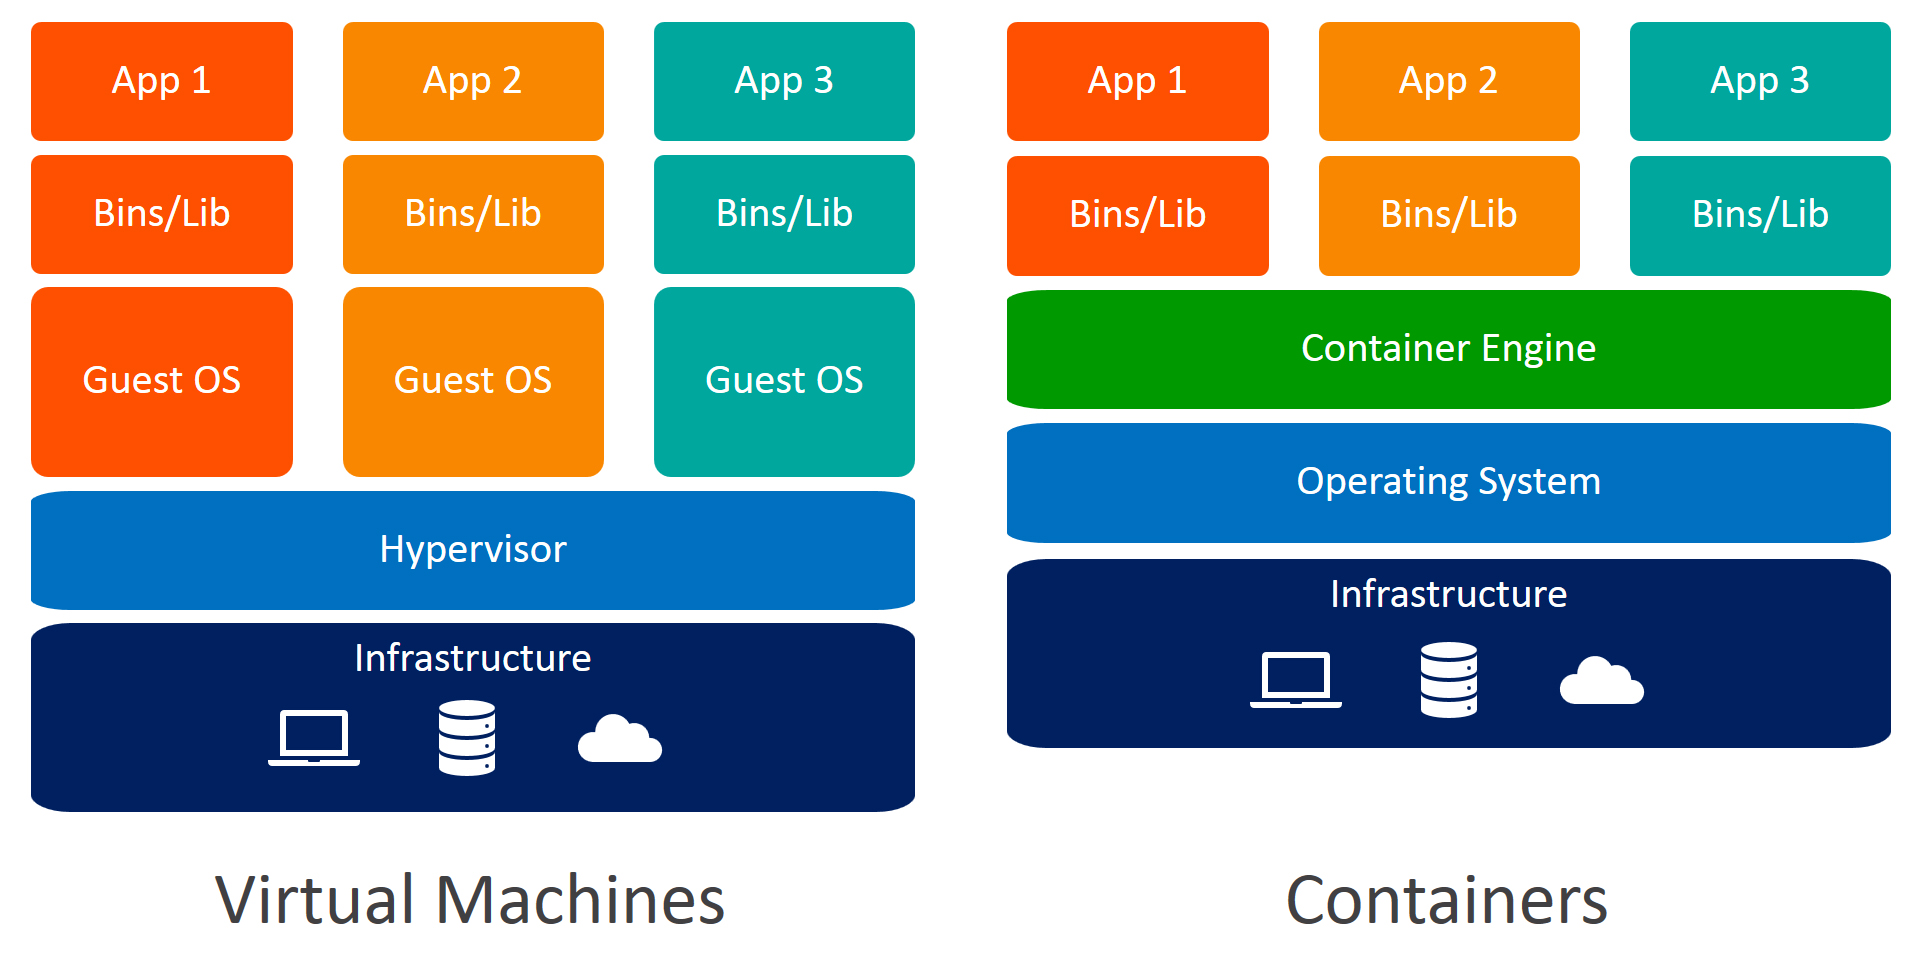
\includegraphics[width=11cm, height=5.5cm]{containers-vs-virtual-machines}
\end{frame}

\section{Container Image}

\subsection{Qué es una Imagen de Container?}

\begin{frame}{Qué es una Imagen de Container?}
 	Básicamente un Container es la instancia de su Imagen.\\
	En la imagen del Container se almacena la configuración del mismo.\\
	En esta configuración se establece el proceso a ejecutar y sus dependencias necesarias, debiéndose especificar las versiones de las mismas. \\
	Esta configuración se almacena en una estructura de árbol.\\
	A partir de una Imagen se puede crear un Contenedor y viceversa, podemos crear y configurar un Contenedor manualmente y luego generar una Imagen. \\
\end{frame}

\subsection{Que es un DockerFile?}
\begin{frame}{Que es un DockerFile?}
	Se denomina DockerFile al archivo en que se almacena la configuracion de una Imagen de Container en Docker. \\
	Luego este archivo se construye en una imagen y se agrega a la lista de imagenes disponibles de Docker para luego poder instanciar un container. \\
\end{frame}

\section{Volumenes}

\subsection{Qué es un Volume?}

\begin{frame}
	Un volumen es una manera de perpetuar los cambios realizados tanto desde el lado del host como del container.\\
	\vspace{.3cm}
	Esto quiere decir que los cambios efectuados en un volumen desde el host se ven reflejados en la imagen del container
	sin necesidad de volverla a crear y permitiendo al container modificar los archivos en un directorio de manera directa\\
\end{frame}

\subsection{Qué es un Bind Mount?}

\begin{frame}
	Un Bind Mount monta una carpeta desde el sistema de archivos local directamente al container. \\
	De esta forma el motor de Docker no puede afectarlo ni reconocerlo directamente. \\
	\vspace{.3cm}
	Ademas los cambios que se realicen a la carpeta desde el container no se van a ver reflejados en el sistema de archivos
	del Host ya que los Bind Mount solo comparten los contenidos de una carpeta. \\
\end{frame}

\subsection{Volumenes vs Bind Mounts}

\begin{frame}
	Volume
	\begin{itemize}
		\item
		Posibilidad del container de modificar directamente los contenidos del volumen.
		\item
		El volumen es creado dentro de una carpeta manejada por el Docker Engine.
		\item
		Accesible desde consola.
	\end{itemize}
	Bind Mount
	\begin{itemize}
		\item
		Consiste en montar un archivo o directorio perteneciente al host, dentro de un container. Este archivo se referencia por su path.
		\item
		Buen rendimiento.
		\item
		Crea dependencias por fuera del Container y del Docker Engine, que no es lo ideal.
		\item
		No puede utilizarse desde la consola de Docker.
		\item
		Rapido despliegue.
	\end{itemize}
\end{frame}

\begin{frame}
	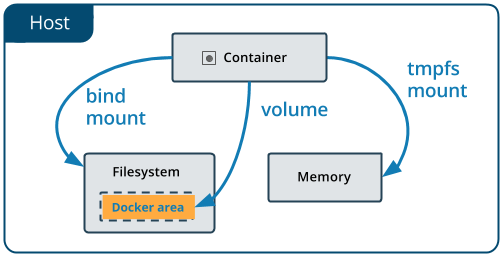
\includegraphics[width=11cm, height=5.5cm]{volume}
\end{frame}

\section{Conexion entre Containers}

\subsection{Introducción}

\begin{frame}{Introducción}
	Como ya sabemos, la idea fundamental de los Containers, es aislar software. Sin embargo, en muchas aplicaciones es necesaria una forma de transmitir información entre Containers, para esto, se crean mecanismos de conexión entre Containers. \\Cabe aclarar que en las siguientes diapositivas se haga referencia a mecanicas específicas a Docker, al ser este el software de Containers en el que nos concentramos.
\end{frame}

\subsection{Cómo se conectan?}
\begin{frame}{Como se conectan los Containers?}
	En la comunicacion entre Containers lo que se hace básicamente es crear una red en la que se expone cada Container como un host. Esto implica que a cada container se le asigna su propia direccion IP y MAC, entre otros parametros.
\end{frame}

\subsection{Red Bridge}
\begin{frame}{Redes: Bridge}
Por defecto todos los containers se conectan a un bridge virtual de Ethernet, en \texttt{Docker} esta representado por la red \texttt{docker0}. Existen otros 2 tipos de redes por defecto en \texttt{Docker}, la red \texttt{host} y la red \texttt{none}
\end{frame}

\subsection{Red Host}

\begin{frame}
\hspace{1cm} La red \texttt{host} añade el Container a la pila de protocolos del Host en el que se ejecuta. Esto significa que no existe ningun tipo de aislamiento entre el Container y el Host, en cuanto a redes se refiere.\\

\hspace{1cm} Esto implica una correspondencia entre los puertos del Container y el Host. \\

\hspace{1cm} Por ejemplo, cualquier servicio ejecutándose en un puerto X del Container, es accesible desde el puerto X del Host. 
\end{frame}

\subsection{Red None}

\begin{frame}
	La red \texttt{none} agrega al Container a una pila de Protocolos específica a dicho Container. En este caso, el Container no tiene una interfaz de red.
\end{frame}

\section{Kubernetes}

\subsection{Que es Kubernetes?}

\begin{frame}{Que es Kubernetes?}
	Kubernetes es una aplicacion que automatiza las tareas manuales relacionadas al despliegue y escabilidad de una aplicacion. \\
	\vspace{.3cm}
	A demas Kubernetes puede administrar multiples host balanceando los niveles de carga entre los hosts y los niveles de demanda
	sobre los containers lanzados en estos. 
\end{frame}


\subsection{Como funciona Kubernetes?}

\begin{frame}{Como funciona Kubernetes?}
	Para funcionar Kubernetes cuenta con una unidad minima llamada Pod. \\
	\vspace{.2cm}
	Un Pod es una abstraccion que permite incluir varios contenedores dentro del mismo elemento y administrar sus requerimientos. \\
	\vspace{.2cm}
	De esta forma, se generan conjuntos de containers autonomos que comparten un Namespace, espacio de IP, etc.
\end{frame}

\begin{frame}{Escabilidad y Confiabilidad}
	Una de las características estrella de Kubernetes es su concepto de replicas. \\
	\vspace{.3cm}
	Precisamente a esto apunta la abstraccion de Containers en Pods; que luego se convertiran en multiples instancias o \texttt{replicas} de una misma aplicacion
	o servicio. \\
	La utilidad de las replicas esta en su aplicacion para Confiabilidad, Balance de Carga y Escalado.
\end{frame}


\subsection{Confiabilidad}

\begin{frame}{Confiabilidad}
	Al tener varias replicas de una aplicacion o servicio, se garantiza el producto final con mayor seguridad, aun si uno o mas de las replicas falla. \\
	\vspace{.3cm}
	Esta es una características muy util en aplicaciones como cloud computing, que estan basadas en la teoria de que uno o mas componentes pueden fallar.
\end{frame}


\subsection{Balance de Carga}

\begin{frame}{Balance de Carga}
	Al tener multiples replicas de un container podemos facilmente distribuir la carga de trabajo efectuada por los usuarios entre las distintas replicas. \\
	\vspace{.3cm}
	Esta características es acompañada a la vez con la posibilidad de utilizar multiples hosts, haciendo asi un mejor uso del hardware disponible.
\end{frame}


\subsection{Escalado}

\begin{frame}{Escalado}
	\hspace{.3cm}Cuando los niveles de carga se elevan demasiado para la cantidad de replicas existentes, Kubernetes permite facilmente escalar la aplicacion
	añadiendo tantas replicas como se requieran para el trabajo.
\end{frame}

\begin{frame}
	Fuentes:
	\begin{itemize}
	\item
	\url{https://www.docker.com/}
	\item
	\url{https://kubernetes.io/es/}
	\item
	\url{https://www.youtube.com/watch?v=iSkkHdGw-C0}
	\item
	\url{https://www.youtube.com/watch?v=TvnZTi_gaNc}
	\item
	\url{https://www.youtube.com/watch?v=EnJ7qX9fkcU}
	\item
	\url{https://www.infoworld.com/article/3204171/what-is-docker-docker-containers-explained.html}
	\end{itemize}
\end{frame}

\end{document}


